\chapter{System Analysis and Design}

\section{System Analysis}

\subsection{Requirement Analysis}

\subsubsection{Functional Requirements}

Key use cases: (1) Submit SOS Request (citizen submits without login; auto-assigned station), (2) Track Request Status (citizen sees real-time status via SSE), (3) Manage Stations/Zones (admin CRUD), (4) Manage Responders (admin account management), (5) View Station Queue (responder sees pending incidents), (6) Claim Incident (responder atomic claim via row-level locking), (7) Update Incident Status (responder marks Arrived/Resolved).

\textbf{Functional Requirements (Summary):}
\begin{itemize}
  \item User authentication (JWT, OAuth2, guest auto-provisioning) with role-based access (Admin, Responder, Citizen).
  \item Station and zone CRUD; zone drawing and GeoJSON upload.
  \item Responder account management and status tracking.
  \item Map visualization of stations and zones (MapLibre GL).
  \item SOS request form with geolocation and category selection.
  \item Automated station assignment via PostGIS zone containment query.
  \item Responder queue view (pending incidents) and task detail view (claimed incident).
  \item Incident lifecycle (Pending → Responding → Arrived → Resolved) with responder action buttons.
  \item Real-time status push via SSE; 5-second polling fallback.
\end{itemize}

\subsubsection{Non-Functional Requirements}

\begin{itemize}
  \item \textbf{Performance:} Spatial triage (ST\_Contains) $< 500$ms; claim operation $< 100$ms under concurrent load.
  \item \textbf{Security:} JWT in HTTP-only cookies; bcrypt password hashing; RBAC on all protected endpoints; row-level locking prevents unauthorized claims.
  \item \textbf{Availability:} Docker health checks; polling fallback maintains eventual consistency if SSE disconnects.
  \item \textbf{Portability:} Single Docker Compose command deploys the entire stack; no external service dependencies.
  \item \textbf{Real-Time Latency:} Status notifications within 1 second (SSE); within 5 seconds (polling).
\end{itemize}

\subsection{Feasibility Analysis}

\textbf{Technical:} Node.js, PostGIS, MapLibre GL, Redis, and SSE are mature open-source tools. Postgres row-level locking is native; spatial queries on GIST-indexed polygons achieve $< 10$ ms latency.

\textbf{Operational:} Citizen SOS flow requires two interactions; admin polygon tool is map-driven; responder dashboard is push-based with minimal polling overhead.

\textbf{Economic:} All dependencies open-source (no licensing cost). Single low-cost VPS deployment with PostgreSQL + Redis.

\textbf{Schedule:} 6 Agile sprints (2-week cycles) completed on schedule; all core objectives delivered.

\begin{figure}[h]
  \centering
  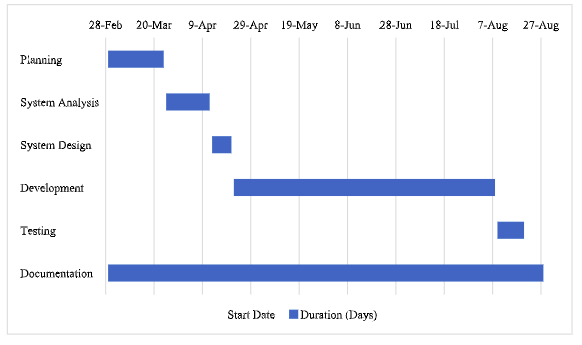
\includegraphics[width=0.95\textwidth]{Graphics/gannt-chart.png}
  \caption{Gantt Chart of Project Timeline}
  \label{fig:gantt}
\end{figure}
\FloatBarrier

\subsection{Object Modelling}

The system's domain model comprises five core classes, each corresponding to a Sequelize ORM model mapped to a database table:

\textbf{Core Classes:} User (authenticated/guest, role-based), Responder (User + station assignment, status tracking), Station (facility with location + category), Zone (service polygon, GIST-indexed for containment queries), Incident (emergency request, lifecycle state + responder assignment).

\begin{figure}[h]
  \centering
  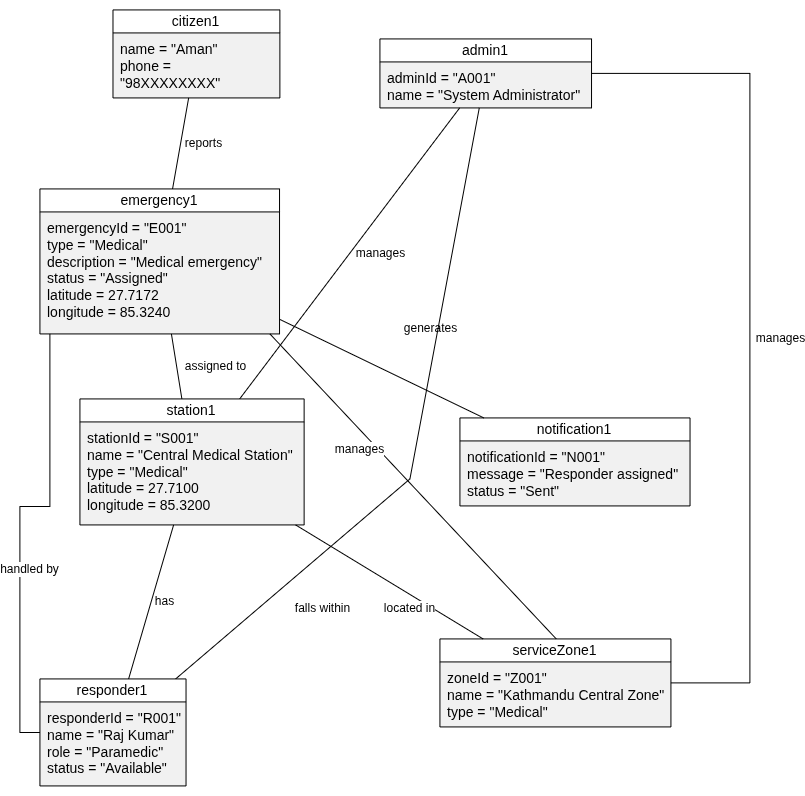
\includegraphics[width=0.6\textwidth]{Graphics/object-diagram.png}
  \caption{Object Diagram - Instance of Incident during active claim (responder 7 on station 3)}
  \label{fig:object}
\end{figure}
\FloatBarrier

\subsection{Dynamic Modelling}

\subsubsection{State Diagram}

\begin{figure}[h]
  \centering
  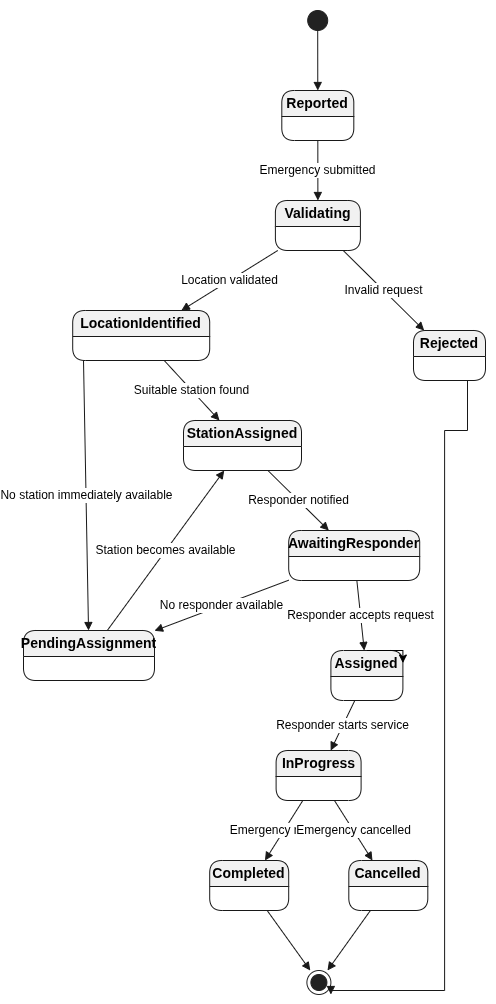
\includegraphics[width=0.55\textwidth]{Graphics/state-diagram.png}
  \caption{State Diagram - Incident lifecycle transitions}
  \label{fig:state}
\end{figure}
\FloatBarrier

Incidents transition through four states: (1) \textbf{Pending}: awaiting responder claim after citizen submission. (2) \textbf{Responding}: responder en route to station, then moving to incident location. (3) \textbf{Arrived}: responder at scene. (4) \textbf{Resolved}: incident handled, responder returns to AVAILABLE. Each transition is atomic and published via Redis pub/sub to subscribed responders and citizens.

\subsubsection{Sequence Diagrams}

\begin{figure}[H]
  \centering
  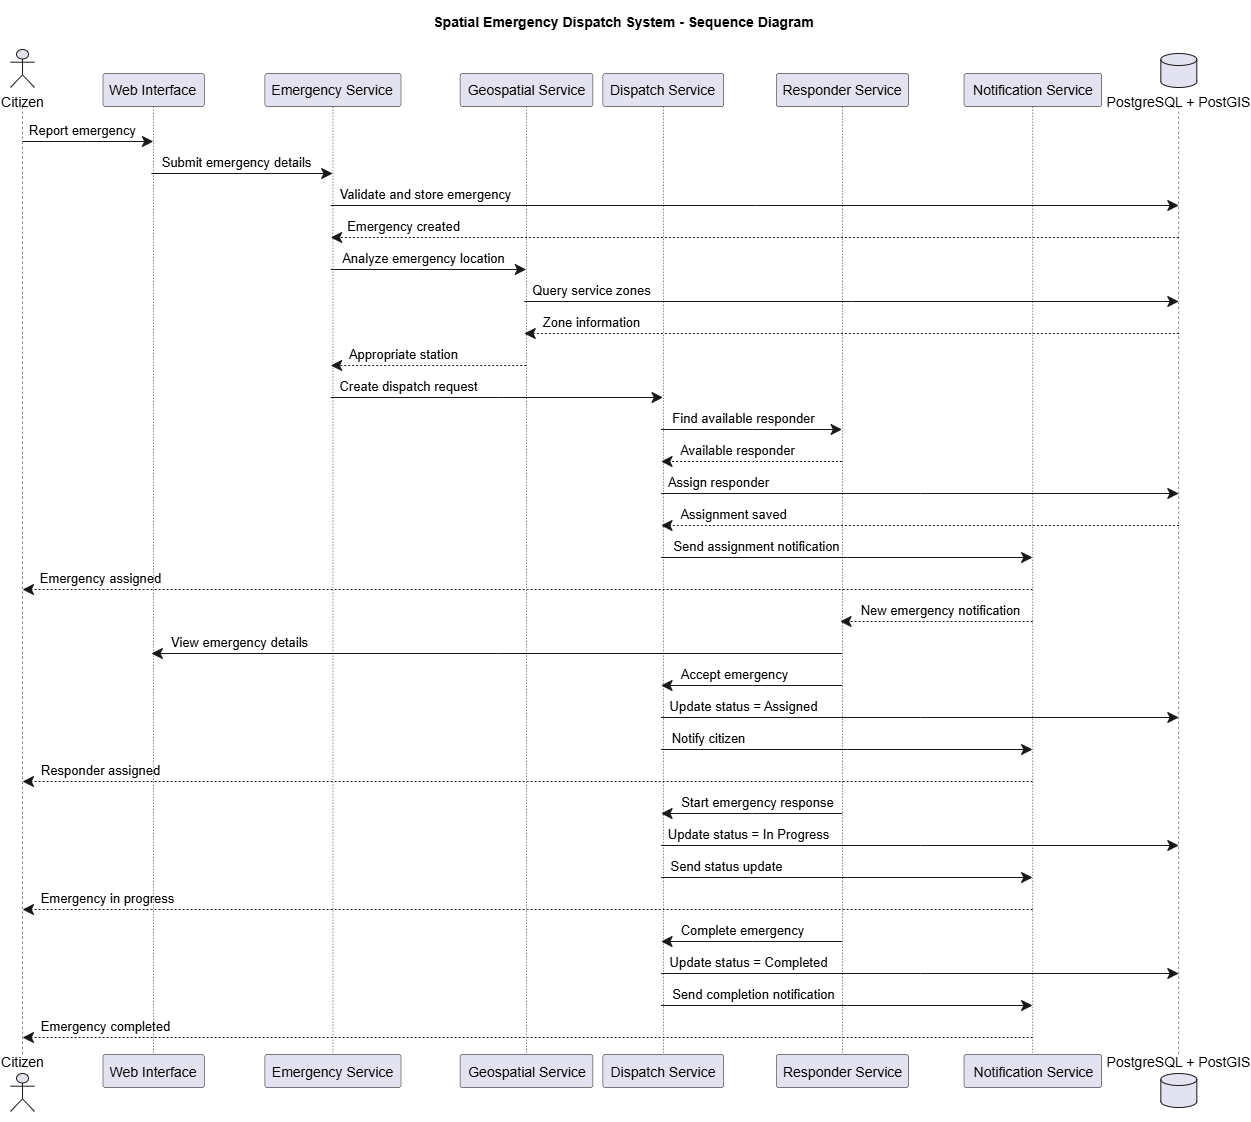
\includegraphics[width=0.95\textwidth]{Graphics/sequence-diagram.png}
  \caption{Sequence Diagram - Spatial Emergency Dispatch System}
  \label{fig:seq-complete}
\end{figure}
\FloatBarrier

The sequence diagram illustrates the complete flow of the emergency dispatch system from citizen SOS submission through responder assignment and emergency completion. It shows interactions between all system components including the Web Interface, Emergency Service, Geospatial Service, Dispatch Service, Responder Service, Notification Service, and the PostgreSQL database with PostGIS.

\subsection{Process Modelling}

\begin{figure}[h]
  \centering
  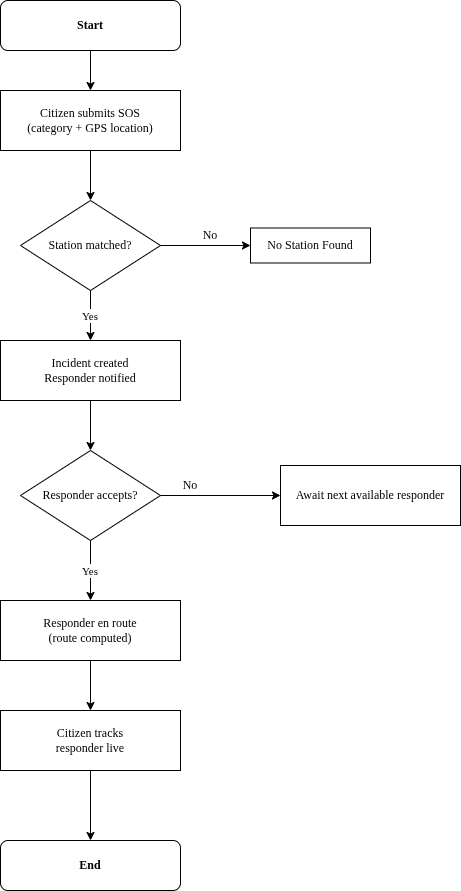
\includegraphics[width=0.45\textwidth]{Graphics/flow.png}
  \caption{Activity Diagram - Incident dispatch process flow from SOS submission through resolution}
  \label{fig:activity-dispatch}
\end{figure}
\FloatBarrier

\section{System Design}

\subsection{Refinement of Class, Object, State, Sequence, and Activity Diagrams}

The analysis-level diagrams above are refined during design with concrete implementation details: class attributes are mapped to database column types and constraints (e.g., zone.boundary is GEOMETRY(Polygon, 4326) with GIST index); methods are decomposed into REST endpoints and database transactions; state transitions are guarded by preconditions (status must be PENDING before claim); sequence flows are augmented with middleware guards (JWT authentication, role checks) and error paths (409 Conflict if claim precondition fails).

\begin{figure}[h]
  \centering
  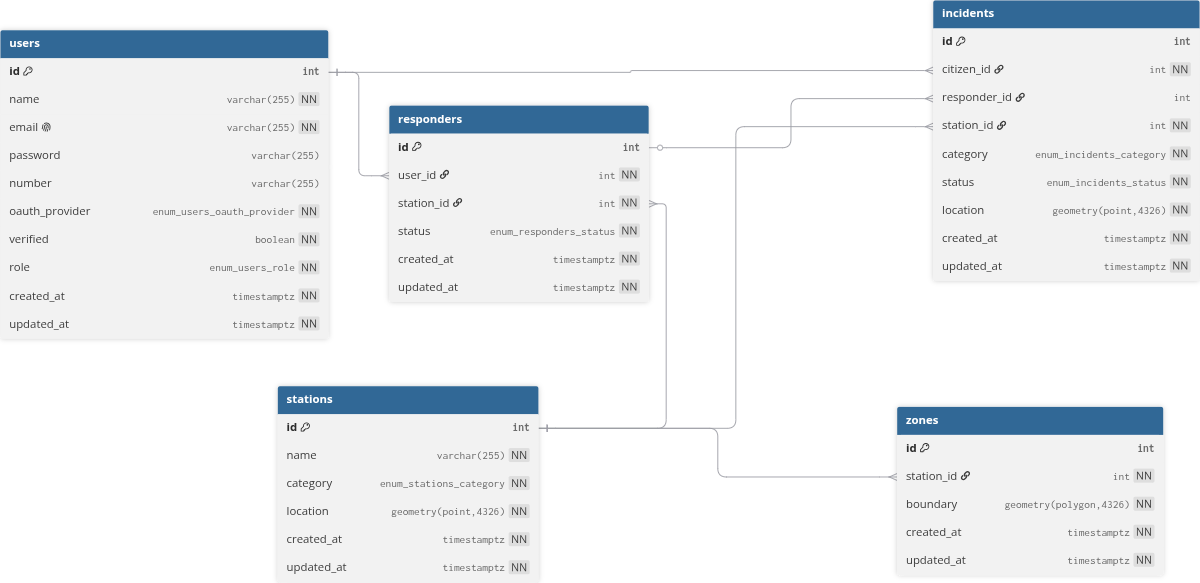
\includegraphics[width=0.95\textwidth]{Graphics/phy_er.png}
  \caption{Refinement of classes and objects diagram of personal finance manager}
  \label{fig:class-refined}
\end{figure}
\FloatBarrier

Schema: \textbf{users} (id, email, password, role), \textbf{stations} (id, name, category, location [POINT]), \textbf{zones} (id, station\_id [FK], boundary [POLYGON, GIST]), \textbf{responders} (id, user\_id [FK], station\_id [FK], status), \textbf{incidents} (id, citizen\_id [FK], station\_id [FK], responder\_id [FK], category, status [PENDING|RESPONDING|ARRIVED|RESOLVED], location [POINT], accepted\_at).

\subsection{System Architecture}

\begin{figure}[h]
  \centering
  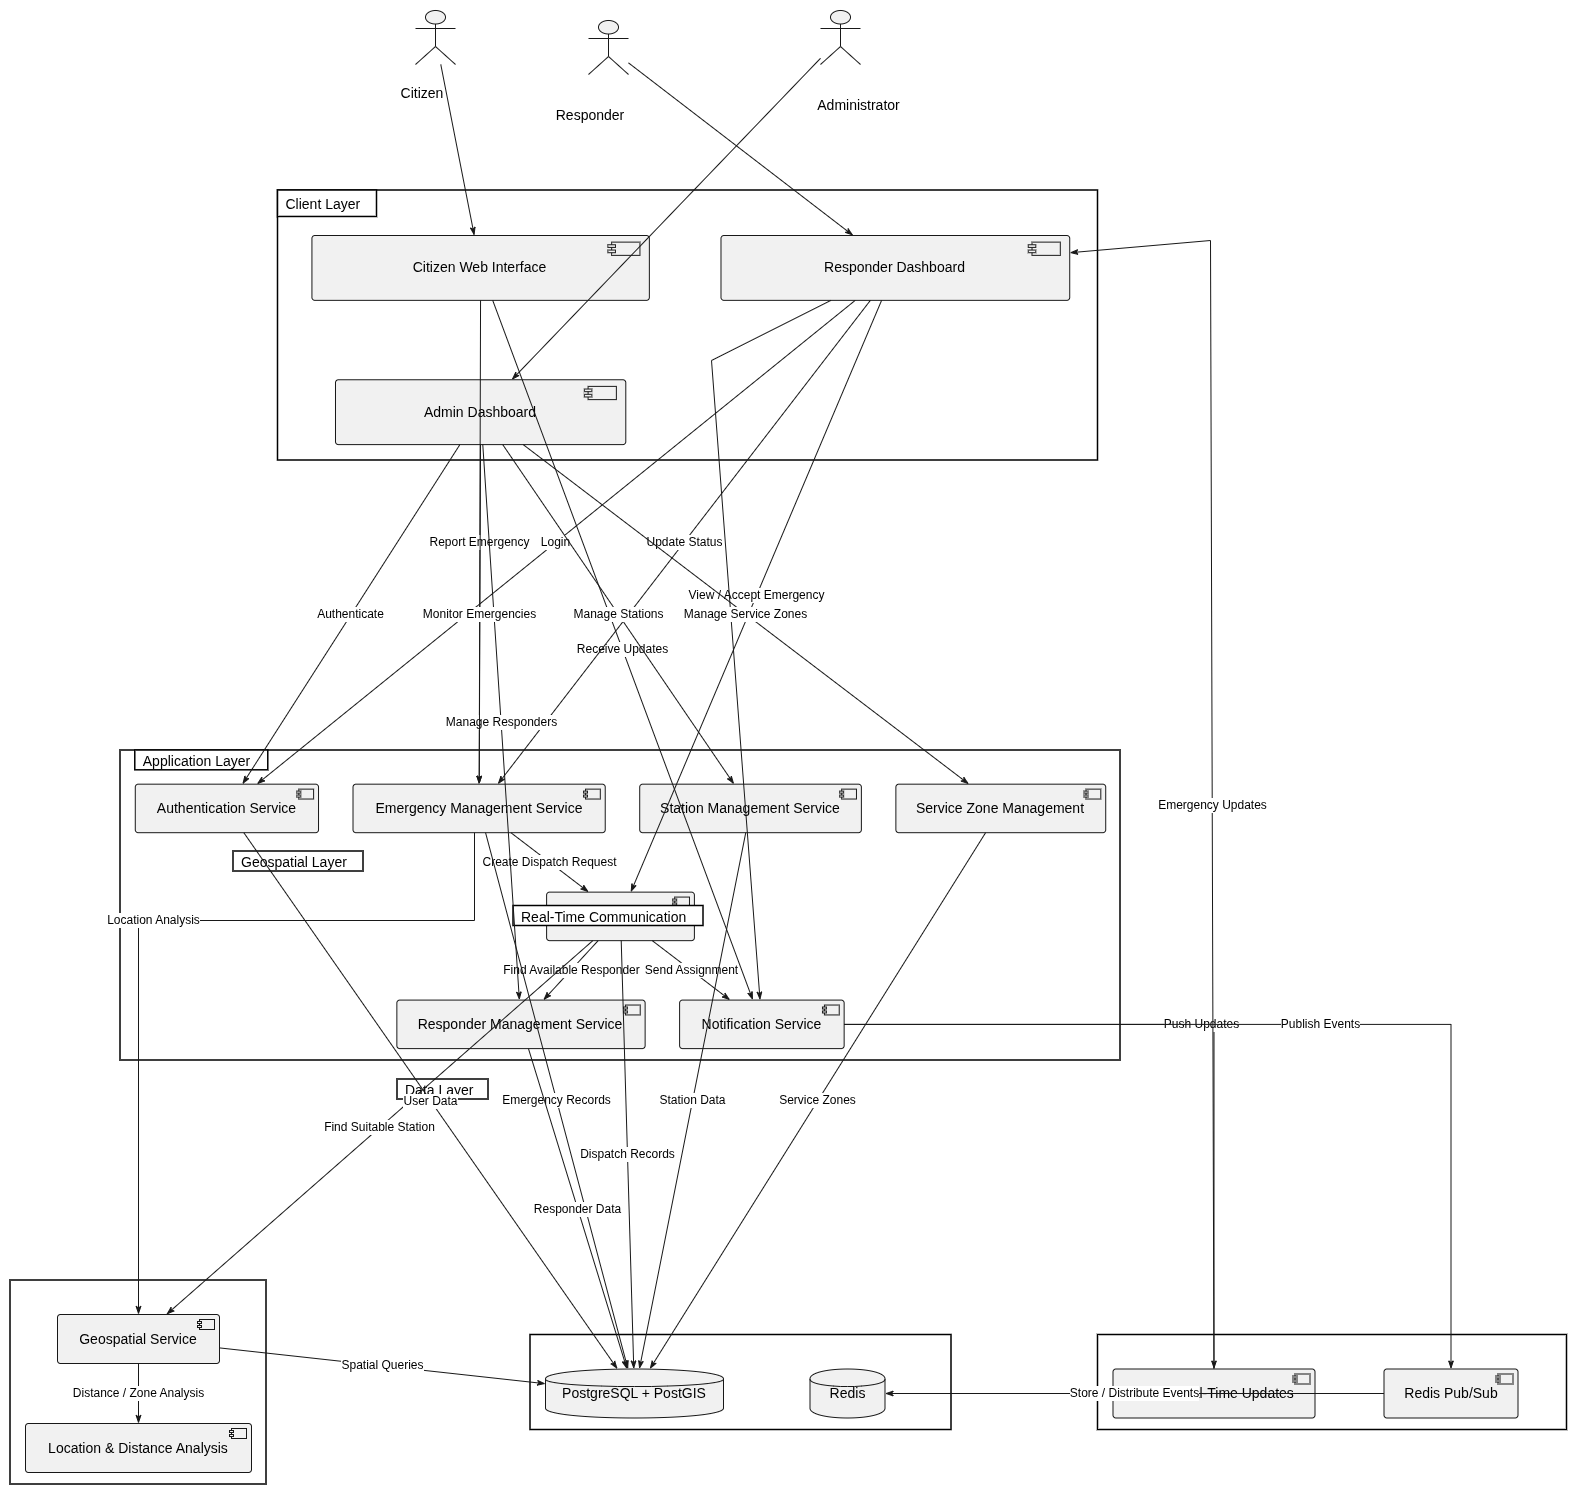
\includegraphics[width=0.75\textwidth]{Graphics/component-diagram.png}
  \caption{Component Diagram - Four-tier architecture with REST/SSE and Pub/Sub}
  \label{fig:component}
\end{figure}
\FloatBarrier
SEDS follows a four-tier architecture: (1) \textbf{Frontend} (Next.js 16, React 19, MapLibre GL, Zustand) on port 3000, communicates with Backend via REST API and SSE streams. (2) \textbf{Backend API} (Node.js 20, Express, Sequelize ORM) on port 9000, handles authentication, incident CRUD, station/zone management, and publishes to Redis pub/sub. (3) \textbf{Redis} (pub/sub broker for ephemeral event fan-out to station and citizen channels; no persistence). (4) \textbf{PostgreSQL 16} (PostGIS 3.4, GIST indexes, row-level locking) for all persistent data.

\subsection{Algorithm Details}

\textbf{Algorithm: A* Pathfinding for Responder Navigation}

SEDS uses the A* algorithm to compute the optimal shortest path from a responder's current location to a citizen's incident location, enabling real-time ETA calculation and turn-by-turn navigation (Step 4 enhancement).

\begin{enumerate}
  \item Input: responder position $p_r = (lng_r, lat_r)$, incident position $p_i = (lng_i, lat_i)$, road network graph $G = (V, E)$ from OpenStreetMap.
  \item Initialize: open set $= \{p_r\}$, closed set $= \emptyset$, $g(p_r) = 0$, $h(p_i) = \text{haversine}(p_r, p_i)$, $f(p_r) = h(p_i)$.
  \item While open set is not empty:
  \begin{enumerate}
    \item Pop node $n$ with lowest $f(n)$.
    \item If $n = p_i$, reconstruct and return path.
    \item For each neighbor $m$ of $n$:
    \begin{enumerate}
      \item Compute $g(m) = g(n) + \text{road\_distance}(n, m)$.
      \item Compute $h(m) = \text{haversine}(m, p_i)$ (admissible heuristic).
      \item If $m$ not in open set, add with $f(m) = g(m) + h(m)$.
      \item Else if $g(m)$ is lower, update $g(m)$ and $f(m)$.
    \end{enumerate}
    \item Add $n$ to closed set.
  \end{enumerate}
  \item Output: Shortest path (list of waypoints), total road distance, estimated time (assuming average responder speed).
\end{enumerate}

A* guarantees optimal shortest path with admissible heuristic. Complexity: $O((V + E) \log V)$ using priority queue. For typical urban road networks (5000 nodes, 10000 edges), computation is $< 100$ ms.
